\documentclass[a4paper,11pt,openany]{book}
%\documentclass[a4paper,twoside,11pt,titlepage]{book}
\usepackage{listings}
\usepackage[utf8]{inputenc}
\usepackage[spanish]{babel}
\usepackage{titlesec}


% \usepackage[style=list, number=none]{glossary} %
%\usepackage{titlesec}
%\usepackage{pailatino}

\decimalpoint
\usepackage{dcolumn}
\newcolumntype{.}{D{.}{\esperiod}{-1}}
\makeatletter
\addto\shorthandsspanish{\let\esperiod\es@period@code}
\makeatother


%\usepackage[chapter]{algorithm}
\RequirePackage{verbatim}
%\RequirePackage[Glenn]{fncychap}
\usepackage{fancyhdr}
\usepackage{graphicx}
\usepackage{afterpage}

\usepackage{longtable}

\usepackage[pdfborder={000}]{hyperref} %referencia

% ********************************************************************
% Re-usable information
% ********************************************************************
\newcommand{\myTitle}{Título del proyecto\xspace}
\newcommand{\myDegree}{Grado en ...\xspace}
\newcommand{\myName}{Nombre Apllido1 Apellido2 (alumno)\xspace}
\newcommand{\myProf}{Nombre Apllido1 Apellido2 (tutor1)\xspace}
\newcommand{\myOtherProf}{Nombre Apllido1 Apellido2 (tutor2)\xspace}
%\newcommand{\mySupervisor}{Put name here\xspace}
\newcommand{\myFaculty}{Escuela Técnica Superior de Ingenierías Informática y de
Telecomunicación\xspace}
\newcommand{\myFacultyShort}{E.T.S. de Ingenierías Informática y de
Telecomunicación\xspace}
\newcommand{\myDepartment}{Departamento de ...\xspace}
\newcommand{\myUni}{\protect{Universidad de Granada}\xspace}
\newcommand{\myLocation}{Granada\xspace}
\newcommand{\myTime}{\today\xspace}
\newcommand{\myVersion}{Version 0.1\xspace}


\hypersetup{
pdfauthor = {\myName (email (en) ugr (punto) es)},
pdftitle = {\myTitle},
pdfsubject = {},
pdfkeywords = {palabra_clave1, palabra_clave2, palabra_clave3, ...},
pdfcreator = {LaTeX con el paquete ....},
pdfproducer = {pdflatex}
}

%\hyphenation{}


%\usepackage{doxygen/doxygen}
%\usepackage{pdfpages}
\usepackage{url}
\usepackage{colortbl,longtable}
\usepackage[stable]{footmisc}
%\usepackage{index}

%\makeindex
%\usepackage[style=long, cols=2,border=plain,toc=true,number=none]{glossary}
% \makeglossary

% Definición de comandos que me son tiles:
%\renewcommand{\indexname}{Índice alfabético}
%\renewcommand{\glossaryname}{Glosario}

\pagestyle{fancy}
\fancyhf{}
\fancyhead[LO]{\leftmark}
\fancyhead[RE]{\rightmark}
\fancyhead[RO,LE]{\textbf{\thepage}}
\renewcommand{\sectionmark}[1]{\markboth{\textbf{\thesection. #1}}{}} % Formato del título de la sección

\setlength{\headheight}{1.5\headheight}

\newcommand{\HRule}{\rule{\linewidth}{0.5mm}}
%Definimos los tipos teorema, ejemplo y definición podremos usar estos tipos
%simplemente poniendo \begin{teorema} \end{teorema} ...
\newtheorem{teorema}{Teorema}[chapter]
\newtheorem{ejemplo}{Ejemplo}[chapter]
\newtheorem{definicion}{Definición}[chapter]

\definecolor{gray97}{gray}{.97}
\definecolor{gray75}{gray}{.75}
\definecolor{gray45}{gray}{.45}
\definecolor{gray30}{gray}{.94}

\lstset{ frame=Ltb,
     framerule=0.5pt,
     aboveskip=0.5cm,
     framextopmargin=3pt,
     framexbottommargin=3pt,
     framexleftmargin=0.1cm,
     framesep=0pt,
     rulesep=.4pt,
     backgroundcolor=\color{gray97},
     rulesepcolor=\color{black},
     %
     stringstyle=\ttfamily,
     showstringspaces = false,
     basicstyle=\scriptsize\ttfamily,
     commentstyle=\color{gray45},
     keywordstyle=\bfseries,
     %
     numbers=left,
     numbersep=6pt,
     numberstyle=\tiny,
     numberfirstline = false,
     breaklines=true,
   }
 
% minimizar fragmentado de listados
\lstnewenvironment{listing}[1][]
   {\lstset{#1}\pagebreak[0]}{\pagebreak[0]}

\lstdefinestyle{CodigoC}
   {
	basicstyle=\scriptsize,
	frame=single,
	language=C,
	numbers=left
   }
\lstdefinestyle{CodigoC++}
   {
	basicstyle=\small,
	frame=single,
	backgroundcolor=\color{gray30},
	language=C++,
	numbers=left
   }

 
\lstdefinestyle{Consola}
   {basicstyle=\scriptsize\bf\ttfamily,
    backgroundcolor=\color{gray30},
    frame=single,
    numbers=none
   }
   
% Define los colores que deseas usar para resaltar el código
\definecolor{mygray}{rgb}{0.5,0.5,0.5}
\definecolor{mygreen}{rgb}{0,0.6,0}
\definecolor{myorange}{rgb}{0.8,0.4,0}
\definecolor{myblue}{rgb}{0,0,0.8}

% Define el estilo para el código JavaScript
\lstdefinestyle{Js}{
    language=Java,
    backgroundcolor=\color{white},   
    commentstyle=\color{mygray},
    keywordstyle=\color{myorange},
    numberstyle=\tiny\color{mygray},
    stringstyle=\color{mygreen},
    basicstyle=\ttfamily\footnotesize,
    breakatwhitespace=false,         
    breaklines=true,                 
    captionpos=b,                    
    keepspaces=true,                 
    numbers=left,                    
    numbersep=5pt,                  
    showspaces=false,                
    showstringspaces=false,
    showtabs=false,                  
    tabsize=1,
    frame=trBL
}


\newcommand{\bigrule}{\titlerule[0.5mm]}


%Para conseguir que en las páginas en blanco no ponga cabecerass
\makeatletter
\def\clearpage{%
  \ifvmode
    \ifnum \@dbltopnum =\m@ne
      \ifdim \pagetotal <\topskip
        \hbox{}
      \fi
    \fi
  \fi
  \newpage
  \thispagestyle{empty}
  \write\m@ne{}
  \vbox{}
  \penalty -\@Mi
}
\makeatother

\usepackage{pdfpages}
\begin{document}
\begin{titlepage}
 
 
\newlength{\centeroffset}
\setlength{\centeroffset}{-0.5\oddsidemargin}
\addtolength{\centeroffset}{0.5\evensidemargin}
\thispagestyle{empty}

\noindent\hspace*{\centeroffset}\begin{minipage}{\textwidth}

\centering

\includegraphics[width=0.9\textwidth]{imagenes/logo_ugr.jpg}\\[1.4cm]

\textsc{ \Large TRABAJO FINAL DE SWAP\\[0.2cm]}
\textsc{ INGENIERÍA INFORMÁTICA}\\[1cm]
% Upper part of the page
% 
% Title
{\Huge\bfseries Cookie Poisoning\\
}
\noindent\rule[-1ex]{\textwidth}{3pt}\\[3.5ex]
{\large\bfseries Servidores Web de Altas Prestaciones} \\
{\large\bfseries Horas Empleadas: 17 horas}
\end{minipage}

\vspace{2.5cm}
\noindent\hspace*{\centeroffset}\begin{minipage}{\textwidth}
\centering

\textbf{Autores}\\ {Daniel Alconchel Vázquez \\
Mario Rodrígues López \\
Sergio Zapata de la Hoz}\\[2.5ex]


\includegraphics[width=0.3\textwidth]{imagenes/etsiit_logo.png}\\[0.1cm]
\textsc{Escuela Técnica Superior de Ingenierías Informática y de Telecomunicación}\\
\textsc{---}\\
Granada, Junio de 2024
\end{minipage}
%\addtolength{\textwidth}{\centeroffset}
%\vspace{\stretch{2}}
\end{titlepage}



%\frontmatter
\tableofcontents
%\listoffigures
%\listoftables
%
\mainmatter
\renewcommand{\thesection}{\arabic{section}} % Asegura numeración arábiga para secciones
\setlength{\parskip}{5pt}

\section{Introducción}

En un mundo donde la tecnología se ha entrelazado con casi todos los aspectos de nuestra vida diaria, la protección de datos y la privacidad se han convertido en preocupaciones primordiales. Desde nuestras interacciones en línea hasta nuestras transacciones financieras, cada acción deja un rastro digital que puede ser explotado si no se maneja adecuadamente.

Imagina por un momento que estás navegando en tu tienda en línea favorita y, sin darte cuenta, alguien está manipulando la información que el sitio web guarda sobre ti. Este proceso, conocido como \textbf{cookie poisoning} o \textbf{envenenamiento de cookies}, es una técnica sutil pero poderosa que los cibercriminales utilizan para robar datos, acceder a cuentas y causar estragos en el mundo digital.

El objetivo de este trabajo es desentrañar los secretos detrás del cookie poisoning. Exploraremos qué son las cookies, cómo pueden ser manipuladas para recopilar información personal sin nuestro conocimiento y consentimiento, y las implicaciones que esto tiene para nuestra privacidad en línea.

¿Te has preguntado alguna vez cómo un atacante puede acceder a tu cuenta sin conocer tu contraseña? ¿O cómo pueden robar tu información personal mientras navegas tranquilamente por internet? Pues sigue leyendo para descubrir cómo protegerte y comprender mejor una de las amenazas más insidiosas del mundo digital moderno.



\clearpage
\section{Antecedentes}

Este apartado revisará la literatura existente y presentará los conceptos fundamentales que sustentan el desarrollo de este trabajo, reforzando la necesidad de estudiar y comprender esta amenaza.

\bigskip

\textbf{Historia y Evolución de las Cookies}

Las cookies fueron introducidas por primera vez en 1994 por Lou Montulli, un programador de Netscape Communications, como una forma de gestionar la información de estado en el navegador web de los usuarios (\cite{kristol2001}). 

Originalmente diseñadas para mejorar la experiencia del usuario al recordar sus preferencias y facilitar el comercio electrónico, las cookies han evolucionado hasta convertirse en una herramienta crucial para la funcionalidad de la web moderna.

\bigskip

\textbf{Conceptos Fundamentales}
\begin{itemize}
    \item \textbf{Cookies}: Pequeños archivos de texto que los sitios web almacenan en el navegador del usuario para recordar información sobre la sesión del usuario, preferencias, y otros datos útiles \cite{rosenblum2001}.

    \item \textbf{Sesiones Web}: Según el estudio de Wang y Goldberg (2006) (\cite{wang2006}), es un mecanismo utilizado por las aplicaciones web para mantener el estado de un usuario entre diferentes solicitudes a un servidor. Las cookies de sesión son fundamentales para este proceso.

    \item \textbf{Protocolo HTTP}: El protocolo HTTP/1.1 se define en el RFC 2616 (Fielding et al., 1999) (\cite{fielding1999}). Se define como un protocolo de solicitud-respuesta utilizado en la comunicación entre el cliente y el servidor en la World Wide Web. 
    
    Funciona como un protocolo sin estado, lo que significa que cada solicitud se procesa de forma independiente, sin conocimiento de solicitudes anteriores. Las cookies se utilizan para mantener el estado de la sesión del usuario entre solicitudes, permitiendo a las aplicaciones web realizar seguimiento del estado de la sesión, recordar preferencias y mantener la autenticación del usuario. 
\end{itemize}

\bigskip

\textbf{Uso de cookies actualmente}

Actualmente los principales usos de las cookies son:

\begin{itemize}
    \item \textbf{Gestión de Sesiones} : Mantienen a los usuarios autenticados mientras navegan por un sitio web, recordando su estado de inicio de sesión.
    \item \textbf{Personalización} : Almacenan preferencias del usuario, como el idioma y temas visuales, mejorando la experiencia de navegación.
    \item \textbf{Análisis y Seguimiento} : Recopilan datos sobre el comportamiento del usuario para análisis de tráfico web y marketing dirigido.
    \item \textbf{Carros de Compra} : Guardan los artículos añadidos en los carros de compras en sitios de comercio electrónico, incluso si el usuario navega fuera del sitio.
\end{itemize}

Puesto que se almacenan datos sensibles es necesario una buena protección de las mismas y es uno de los temas que discutiremos posteriormente en este trabajo.






\clearpage
\section{Objetivos}

A modo de resumen, este proyecto consiste en explorar y comprender el envenenamiento de cookies, así como identificar sus mecanismos, riesgos y medidas de protección, y realizar una prueba práctica para evaluar la efectividad de las estrategias de mitigación propuestas.

\bigskip

\textbf{Desglose de Objetivos}
\begin{enumerate}
    \item {\textbf{Definir y explicar el concepto de envenenamiento de cookies, incluyendo sus métodos y técnicas comunes.}
    \begin{itemize}
        \item Describir las diferentes formas en que se puede realizar el envenenamiento de cookies.
        \item Identificar las vulnerabilidades que hacen posible este tipo de ataque.
    \end{itemize} }

    \item {\textbf{Analizar casos reales y estudios de envenenamiento de cookies para ilustrar la gravedad y las consecuencias de estos ataques.}
    \begin{itemize}
        \item Revisar incidentes documentados y reportes de seguridad.
        \item Evaluar el impacto de estos ataques en diferentes sectores y aplicaciones web.
    \end{itemize} }

    \item {\textbf{Examinar y evaluar las técnicas y herramientas existentes para la prevención y detección del envenenamiento de cookies.}
    \begin{itemize}
        \item Investigar las mejores prácticas de seguridad recomendadas para proteger las cookies.
        \item Comparar diferentes enfoques y tecnologías utilizadas para mitigar estos riesgos.
    \end{itemize} }

    \item {\textbf{Realizar una prueba práctica que simule un ataque de envenenamiento de cookies y evaluar la eficacia de las medidas de protección implementadas.}
    \begin{itemize}
        \item Diseñar y llevar a cabo un experimento controlado que reproduzca un escenario de envenenamiento de cookies.
        \item Medir y analizar los resultados para determinar la efectividad de las estrategias de mitigación propuestas.
    \end{itemize} }

    \newpage

    \item {\textbf{Documentar y presentar los hallazgos del trabajo, proporcionando conclusiones y sugerencias para futuras investigaciones en el área de la ciberseguridad relacionada con las cookies.}
    \begin{itemize}
        \item Resumir los resultados obtenidos y su relevancia para la comunidad de ciberseguridad
        \item Ofrecer recomendaciones para estudios futuros y posibles mejoras en las técnicas de protección.
    \end{itemize} }
\end{enumerate}

Estos objetivos están estructurados para proporcionar un análisis completo y detallado del envenenamiento de cookies, desde su comprensión teórica hasta la aplicación práctica de medidas de seguridad, culminando en una prueba práctica que validará la investigación realizada.


\clearpage
\section{Desarrollo de los objetivos}

\subsection{¿Qué es el envenenamiento de cookies? Conceptos y métodos utilizados}

Como bien hemos hablado antes en los antecedentes, las cookies son datos específicos de un sitio web, que incluyen información de interés sobre los usuarios y que se almacenan en sus navegadores. Se utilizan principalmente para rastrear tendencias de uso, personalizar la experiencia de una web, etc...

Los atacantes pueden interceptar estas cookies antes de que vuelvan al servidor para extraer información de ellas o modificarlas. Las cookies también pueden ser falsificadas creando una desde cero como un medio de hacerse pasar por un usuario para acceder a datos adicionales de estos. Por tanto, el \textbf{cookie poissoning} es el nombre que recibe al conjunto de métodos utilizados para robar datos de las cookies de los usuarios u otros usos con intenciones maliciosas sobre las mismas.

Principalmente se usa esta técnica para la suplantación de identidad. Uno de los principales usos de las cookies es la autenticación, ya que contienen información que permite a los usuarios navegar sin estar autenticándose constantemente, por lo que la técnica de envenenamiento de cookies es un método recurrido por los atacantes para robar la identidad de los usuarios, con el objetivo de conseguir acceso no autorizado a un servidor web o para realizar fraude.

Algunos de los medios y técnicas que permiten a los atacantes realizar este tipo de ataques son los siguientes (\cite{techtarget2024cookie}, \cite{accessq2024envenenamiento}):

\begin{itemize}
    \item \textbf{Manipulación de cookies del lado del cliente:} Los atacantes pueden usar herramientas de desarrollo del navegador para modificar manualmente el contenido de las cookies o usar plugins que permitan la manipulación automática de las mismas.

    \item \textbf{Intercepción del tráfico:} Los atacantes pueden interceptar el tráfico de red, pudiendo capturar y modificar las cookies en tránsito, especialmente si no están cifradas (muy común cuando se usa el protocolo \texttt{HTTP} en lugar de \texttt{HTTPs}). A esta técnica de interceptar la comunicación entre un cliente y un servidor se le conoce como \textbf{Man in the Middle}.

    \item \textbf{Inyección de scripts (Cross-Site-Scripting - XSS):} Los atacantes pueden hacer uso de las vulnerabilidades que presentan las webs que estén ejecutando un software inseguro, mediante la inserción de scripts maliciosas que permitan obtener estos datos.
\end{itemize}

Dado estos distintos tipos de técnicas, podemos diferenciar entonces entre los siguientes tipos de cookie poissoning (\cite{appsecmonkey2024session}, \cite{ibm2024cookie}):

\begin{itemize}
    \item \textbf{Cookie Overwriting:} Es cuando el atacante fuerza al navegador del usuario a aceptar una cookie modificada, remplazando la original, normalmente mediante la inserción de scripts maliciosas en un sitio web.

    \item \textbf{Session Fixation:} El atacante establece una cookie de sesión específica en el navegador del usuario y luego, a través del uso de técnicas de ingeniería social o enlaces maliciosos, induce al usuario a autenticarse. De esta forma, el atacante recibe los datos de dicha autenticación, permitiéndole suplantar la identidad del usuario.

    \item \textbf{Cookie Hijacking:} El atacante roba una cookie válida de un usuario (por ejemplo, mediante XSS) y la usa para suplantar su identidad.

    \item \textbf{Cookie Replay:} El atacante reutiliza una cookie válida capturada previamente para repetir una acción autorizada. Esto es posible cuando los servidores no verifican adecuadamente la temporalidad y unicidad de las cookies.
\end{itemize}

Hemos visto los distintos tipos de cookie poissoning existentes y las técnicas usadas en las mismas, pero, ¿cómo es posible que ocurra este tipo de ataques? Algunas de las razones que permiten a los atacantes realizar este tipo de ataques son la \textbf{falta de cifrado (Uso de HTTP en lugar de HTTPs)}, que permite que las cookies sean mucho más fáciles de interceptar al no estar cifradas; el uso de \textbf{cookies no seguras}, que son aquellas que no usan los flags de \texttt{Secure}\footnote{Asegura que las cookies solo se envíen mediante conexiones HTTPs} y \texttt{HttpOnly}\footnote{Impide el acceso a la cookie mediante JavaScript, mitigando el riesgo XSS}; la \textbf{validación inadecuada del lado del servidor}, la reutilización de tokens de sesión, la falta de expiración adecuada de las cookies de sesión u otras vulnerabilidades de la aplicación web en cuestión.

\subsection{Análisis de casos reales}

Para comprender mejor la gravedad y las consecuencias del envenenamiento de cookies, es útil analizar casos reales. Algunos casos conocidos son los siguientes:

\begin{itemize}
    \item \textbf{Ataque a Yahoo (2014-2016) \cite{bbc2016noticias}}: Entre 2014 y 2016, Yahoo fue víctima de un masivo ataque de envenenamiento de cookies que comprometió más de 3 mil millones de cuentas de usuarios. Los atacantes utilizaron técnicas avanzadas para crear cookies falsificadas que permitieron el acceso a las cuentas de usuario sin necesidad de conocer las contraseñas. Este incidente afectó gravemente a la reputación de Yahoo, que ya estaba en negociaciones para ser adquirida por Verizon. La noticia del ataque redujo el valor de la adquisición en varios cientos de millones de dólares. Además, supuso un compromiso de información personal, como correos electrónicos, contactos, etc...

    \item \textbf{Exploit de Microsoft ASP.NET (2010)}: En 2010, se descubrió una vulnerabilidad en el framework ASP.NET de Microsoft que permitía a los atacantes realizar envenenamiento de cookies para obtener datos sensibles. El exploit, conocido como "Padding Oracle Attack," permitía a los atacantes descifrar datos encriptados en cookies y otros campos. Esta vulnerabilidad podía ser explotada para acceder a información cifrada, comprometiendo potencialmente millones de aplicaciones web basadas en ASP.NET.

    \item \textbf{Ataque de envenenamiento de cookies a LastPass (2022) \cite{unaaldia2022lastpass}} : Un ataque de envenenamiento de cookies permitió a los ciberdelincuentes acceder a las cuentas de LastPass de los usuarios y robar sus contraseñas.

    \item \textbf{Vulnerabilidad en Shopify (2017)}: En 2017, se descubrió una vulnerabilidad en la plataforma de comercio electrónico Shopify que permitía el envenenamiento de cookies a través de un exploit de inyección de código. Este ataque podría haber permitido a los atacantes hacerse pasar por otros usuarios, accediendo a sus cuentas y datos personales. Aunque la vulnerabilidad fue rápidamente parcheada, el riesgo de comprometer datos financieros y personales de comerciantes y clientes de Shopify era significativo.

    \item \textbf{Ataque de envenenamiento de cookies a Barneys New York (2014)} : Un ataque de envenenamiento de cookies permitió a los ciberdelincuentes robar información personal de los clientes de Barneys New York, incluyendo nombres, direcciones, números de teléfono y direcciones de correo electrónico.

    \item \textbf{Estudio de la Universidad de California en Berkeley (2016)} : Un estudio de la Universidad de California en Berkeley encontró que el 70\% de los sitios web populares eran vulnerables a ataques de envenenamiento de cookies.
\end{itemize}

\newpage

\subsection{Detección y Prevención}

Vamos ahora a estudiar algunas técnicas de prevención y detección del envenenamiento de cookies (\cite{linkedin2024cookie}, \cite{f52024cookie}, \cite{linkedin2024cookie2}). Alguna de las medidas más utilizadas son las siguientes:

\begin{itemize}
    \item \textbf{Uso de HTTPs} : Pese a que la configuración de https para los sitios web es una tarea más compleja que el simple uso de http, permite aumentar en gran medida la seguridad de la misma; en especial ayuda a prevenir la interceptación y manipulación de las cookies durante su transmisión.

    \item \textbf{Cookies Seguras (\texttt{Secure} y \texttt{HrrpOnly)}}: Ya hemos visto previamente estos conceptos. El uso de este tipo de cookies permite que solo se transmitan mediante https y mitigan los ataques de tipo XSS.

    \item \textbf{Implementar cookies en el mismo sitio} : Otra forma de evitar el robo de cookies es implementar cookies del mismo sitio, que restringen el alcance de las cookies al mismo dominio o subdominio que la aplicación web. Esto evita que los atacantes exploten las vulnerabilidades de falsificación de solicitudes entre sitios.

    \item \textbf{Supervisar y expirar sesiones} : Para detectar y responder al robo de cookies, también debe supervisar y caducar las sesiones de su aplicación web. Puede utilizar identificadores de sesión, marcas de tiempo, direcciones IP, agentes de usuario y otros atributos para realizar un seguimiento de la actividad y la validez de sus sesiones. También puede establecer un breve tiempo de expiración para sus sesiones y cookies, y solicitar a los usuarios que se vuelvan a autenticar periódicamente o después de ciertas acciones. De esta manera, puede reducir la ventana de oportunidad para que los atacantes utilicen cookies robadas e invalidarlas si detecta alguna anomalía o comportamiento sospechoso.

    \item \textbf{Políticas de Seguridad de Contenidos (CSP)} : Implementar políticas de seguridad para controlar cómo se carga y ejecuta el contenido web, ayudando de esta forma a prevenir ataques de inyección de código que podrían modificar las cookies.

    \item \textbf{Validación de cookies en el servidor} : Otra medida recomendada es implementar validaciones en el servidor que aseguren que las cookies no hayan sido alteradas.

    \item \textbf{Cookies firmadas y encriptadas} : Usar este tipo de cookies permite garantizar su integridad y confidencialidad, impidiendo su modificación y lectura por parte de los atacantes.
\end{itemize}

Además de estas medidas que son configurables e integrables por parte de los programadores, se pueden usar tras herramientas externas que ayuden a aumentar la seguridad de nuestra web, así como la detección de este tipo de ataques. Algunas de estas herramientas externas son los \textbf{Web Application Firewalls (WAFs)}, que permiten filtrar y monitorizar el tráfico HTTP hacia y desde una aplicación web para detectar y mitigar ataques, \textbf{herramientas de auditoría de seguridad}, como \texttt{Burp Suite} o \texttt{OWASP ZAP}, que permiten detectar vulnerabilidades en nuestra aplicación web, las cuales podrían ser utilizadas para el cookie poisoning o el uso de \textbf{Intrusion Detection Systems (IDS)}, como \texttt{Snort}, para monitorizar la red y los sistemas en busca de actividad sospechosa.

Incluso con todas estas herramientas, a día de hoy se siguen buscando nuevas formas de combatir este tipo de ataque. Hace pocos días \texttt{Google} anunció que está trabajando en nuevas medidas de seguridad. Está desarrollando una nueva función de seguridad para Chrome llamada \textbf{Credenciales de Sesión Vinculadas al Dispositivo (DBSC)} [\cite{bitlifemedia2024google}, \cite{escudodigital2024google}] para combatir el robo de cookies de sesión y el acceso no autorizado a cuentas de usuario. Esta función vincula las sesiones de autenticación al dispositivo del usuario, haciendo que las cookies robadas sean inútiles para los atacantes, a menos que puedan operar localmente en el dispositivo comprometido. DBSC utiliza un par de claves pública/privada generadas localmente en el dispositivo, protegiendo la clave privada mediante TPMs y considerando soluciones aisladas por software. Cada sesión está asociada con una clave pública, y los servidores verifican la correspondencia de la clave privada para garantizar la continuidad del acceso. Además, DBSC mantiene las cookies de corta duración a través de un punto final definido por DBSC en el sitio web, reduciendo los cambios necesarios en sitios web y aplicaciones. Esta solución respeta la privacidad de los usuarios al no permitir la correlación de claves entre sesiones en el mismo dispositivo, y permite a los usuarios eliminar las claves cuando lo deseen. Google espera que DBSC se convierta en un estándar web abierto, colaborando con proveedores de servidores, IdPs y navegadores para presentar un estándar que preserve la privacidad y mejore la seguridad en internet.

Por último, también es aconsejable que se eduque a la población para que sea consciente de este tipo de problemas. Vivimos en una era digitalizada, donde todo el mundo usa, transmite y publica datos por la red; pero son pocas las personas que son conscientes de los peligros que existen en la misma y de las malas prácticas que deben evitar.

\subsection{Prueba práctica}

A continuación vamos a realizar una pequeña prueba práctica de interceptación de cookies. Todo se realizará en un entorno controlado y local. Además, iremos detallando paso a paso el experimento para que pueda ser replicado por cualquiera. 

\textit{En nuestro caso estamos usando \texttt{Ubuntu 22.0} para la prueba y el navegador \texttt{FireFox}. Usar otro sistema o navegador puede alterar ligeramente alguno de los pasos de configuración, pero el proceso sigue siendo el mismo salvo ajustes.}

Comenzamos creando una carpeta para el proyecto. Una vez creada y accedido a dentro del directorio, vamos a usar \texttt{Node.js} para crear un pequeño servidor web (\textit{Si no tienes esta herramienta, puedes instalarla desde este \href{https://nodejs.org/en/download/package-manager}{enlace}}).

Para crear el proyecto usamos los siguientes comandos:

\begin{lstlisting}[style=Consola]
    # Inicializa un nuevo proyecto de Node.js
    npm init -y
    
    # Instala Express
    npm install express cookie-parser
\end{lstlisting}

Lo siguiente es crear el servidor. Para ello, creamos el archivo \texttt{server.js} y añadimos el siguiente contenido:

\begin{lstlisting}[style=Js]
    const express = require('express');
    const cookieParser = require('cookie-parser');
    const app = express();
    
    app.use(cookieParser());
    app.use(express.json());
    
    const PORT = 3000;
    
    // Middleware para verificar autenticacion
    function checkAuth(req, res, next) {
        const userCookie = req.cookies.user;
        if (userCookie) {
            const user = JSON.parse(userCookie);
            req.user = user;
            next();
        } else {
            res.status(401).send('No estas autenticado');
        }
    }
    
    // Ruta de login
    app.post('/login', (req, res) => {
        const { username, role } = req.body;
        if (username && role) {
            const user = { username, role };
            res.cookie('user', JSON.stringify(user), { httpOnly: true });
            res.send('Inicio de sesion exitoso');
        } else {
            res.status(400).send('Faltan parametros');
        }
    });
    
    // Ruta protegida
    app.get('/admin', checkAuth, (req, res) => {
        if (req.user.role === 'admin') {
            res.send(`Bienvenido, admin ${req.user.username}`);
        } else {
            res.status(403).send('Acceso denegado');
        }
    });
    
    // Ruta publica
    app.get('/', (req, res) => {
        res.send('Pagina publica');
    });
    
    app.listen(PORT, () => {
        console.log(`Servidor escuchando en http://localhost:${PORT}`);
    });
\end{lstlisting}

Como podemos observar, es un código muy sencillo con 3 endpoints. El path \texttt{/} define la página principal y muestra el texto "Página pública". El path \texttt{/login} está configurado para recibir peticiones \texttt{POST} y permite iniciar sesión al usuario. Por último, el path \texttt{/admin} muestra la página sólo si somos administradores, en caso contrario nos devuelve un error \texttt{403}, indicando que no tenemos permisos.

Para levantar el servidor, simplemente ejecutamos el siguiente comando desde la terminal:

\begin{lstlisting}[style=Consola]
    node server.js
\end{lstlisting}

Puedes acceder a la web desde el navegador usando la url \\ \texttt{http://localhost:3000}.

\newpage

A continuación, vamos a usar el navegador para mandar una solicitud \texttt{POST} a \texttt{http://localhost:3000/login} con el siguiente cuerpo \texttt{JSON}:

\begin{verbatim}
    {
        "username": "usuario1",
        "role": "user"
    }
\end{verbatim}

Esto creará una cookie de usuario con el rol ''user''. Luego, intenta acceder a \texttt{http://localhost:3000/admin}. Deberías observar el texto `Acceso Denegado`.

\begin{center}
    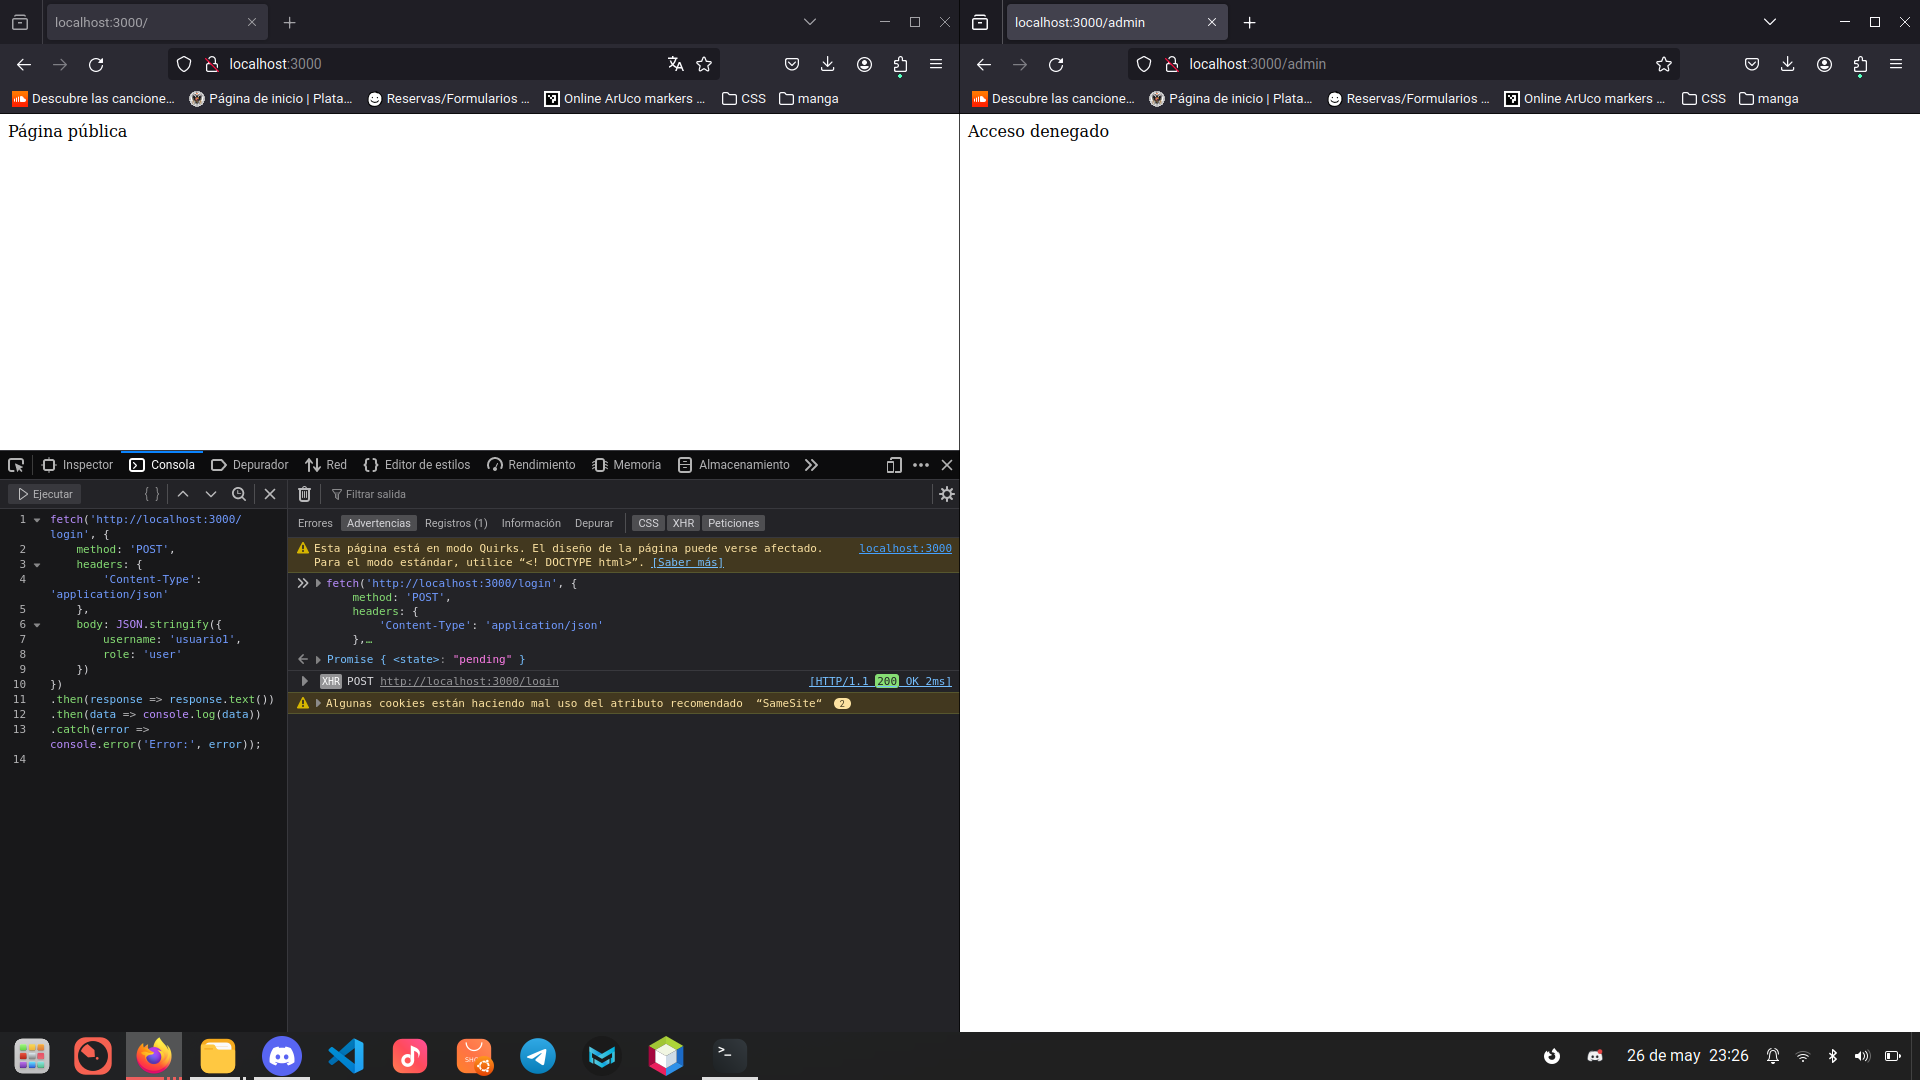
\includegraphics[scale=0.18]{imagenes/Captura desde 2024-05-26 23-26-34.png}
\end{center}

\textit{Para mandar la solicitud \texttt{POST} desde la consola del navegador puedes usar el siguiente código}:

\begin{figure}[h]
\begin{lstlisting}[style=Js, label={lst:fetch-post}]
fetch('http://localhost:3000/login', {
    method: 'POST',
    headers: {
        'Content-Type': 'application/json'
    },
    body: JSON.stringify({
        username: 'usuario1',
        role: 'user'
    })
})
.then(response => response.text())
.then(data => console.log(data))
.catch(error => console.error('Error:', error));
\end{lstlisting}
\end{figure}

\newpage

A continuación, vamos a instalar \href{https://portswigger.net/burp/communitydownload}{\texttt{Burp Suite Community Edition}} para interceptar el tráfico y usarlo como proxy del navegador. Para instalarlo, sigue los pasos del link anterior.

Una vez instalados, podemos abrir el programa y creamos un proyecto temporal. Una vez dentro de la interfaz, nos vamos al apartado de \texttt{Proxy > Proxy Settings} y establecemos la siguiente configuración:

\begin{center}
    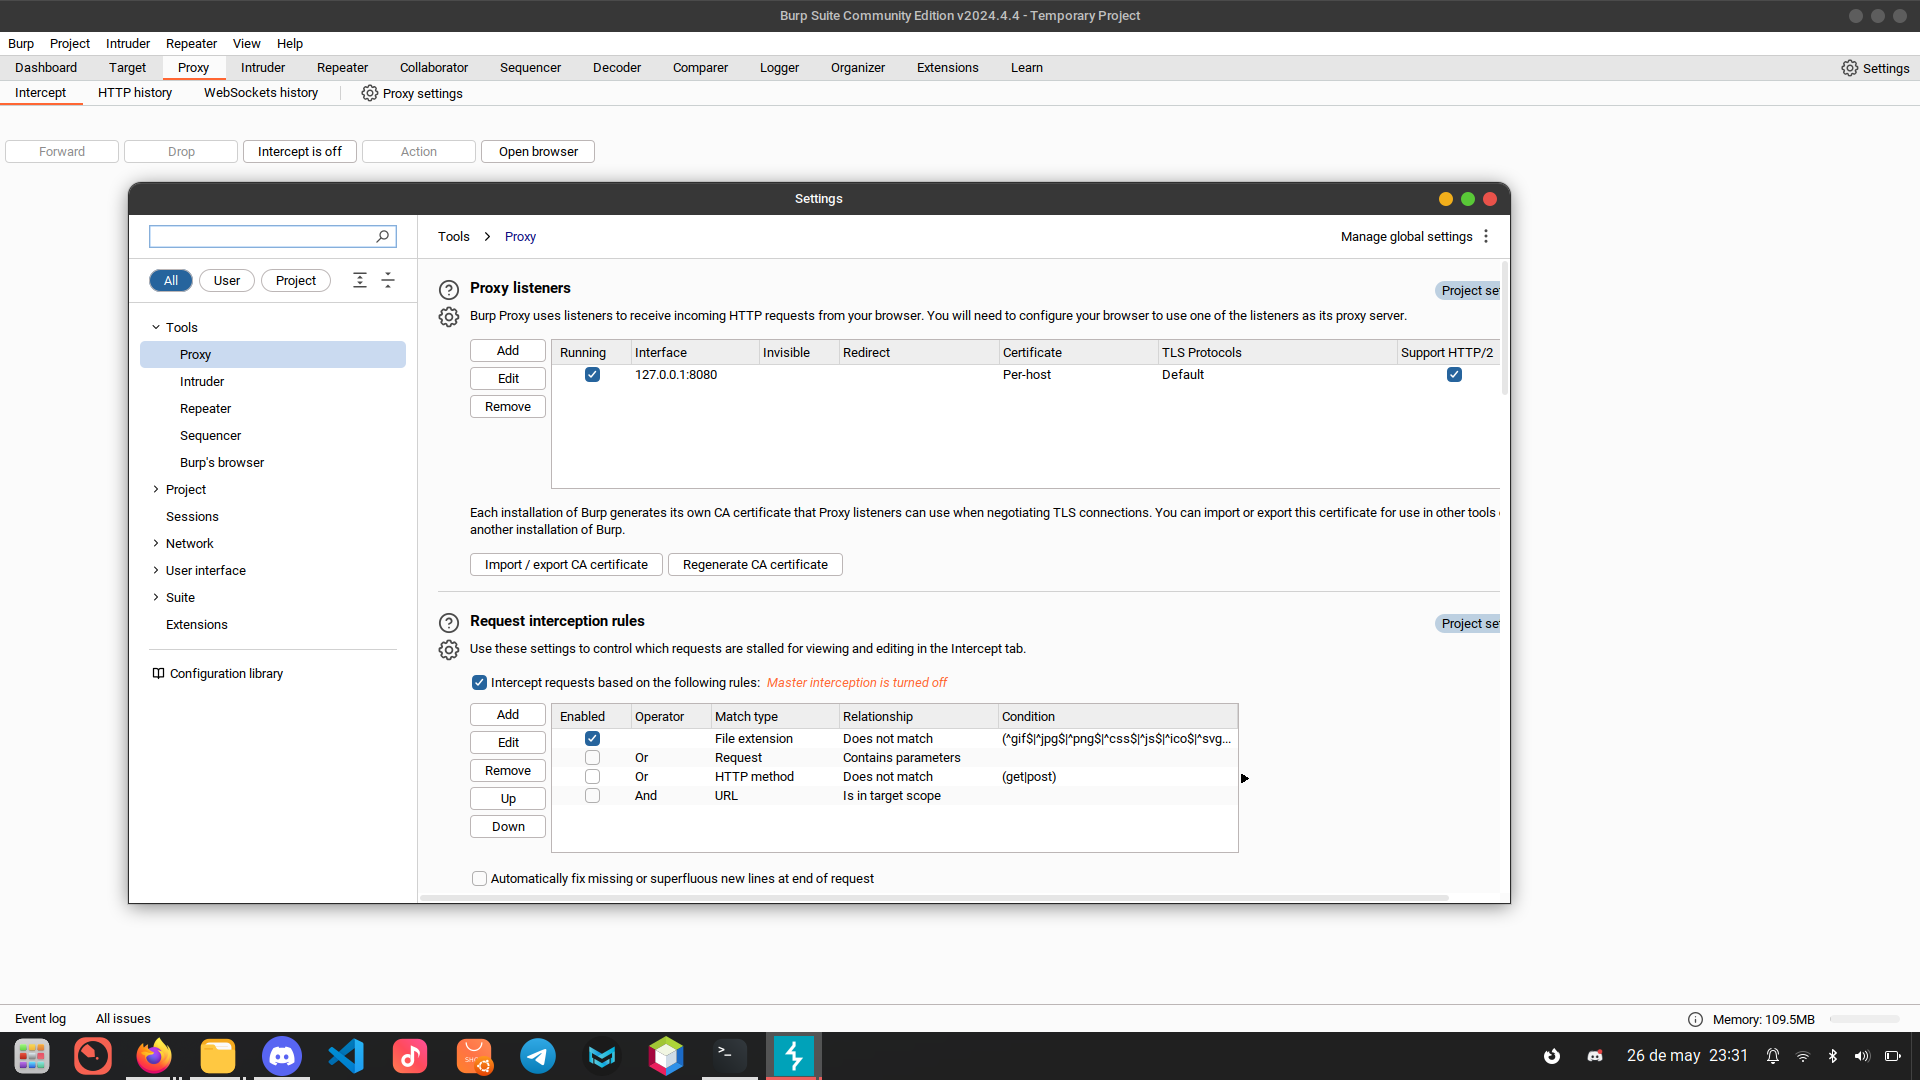
\includegraphics[scale=0.18]{imagenes/Captura desde 2024-05-26 23-31-47.png}
\end{center}

A continuación, vamos al navegador. En nuestro caso estamos utilizando \texttt{FireFox}, por lo que habrá que configurar unas cuantas cosas:

\begin{enumerate}
    \item \textbf{Habilitar el proxy para localhost, el cual viene desactivado por defecto}: Para ello, simplemente escribimos \texttt{about:config} en la url y buscamos la siguiente configuración, la cual, debemos establecer a \texttt{true}:

    \begin{center}
        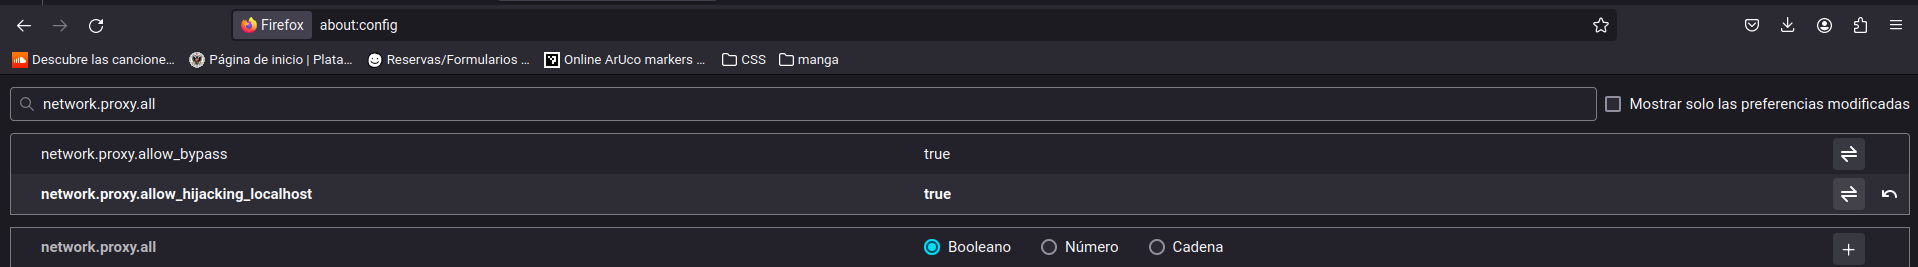
\includegraphics[scale=0.17]{imagenes/Captura desde 2024-05-26 22-29-09.png}
    \end{center}

    \item \textbf{Establecer Burp Suite como proxy} : Ve a la ventana de \texttt{Ajustes} de FireFox y busca \texttt{Configuración de red}. Allí, establece la siguiente configuración:

    \begin{center}
        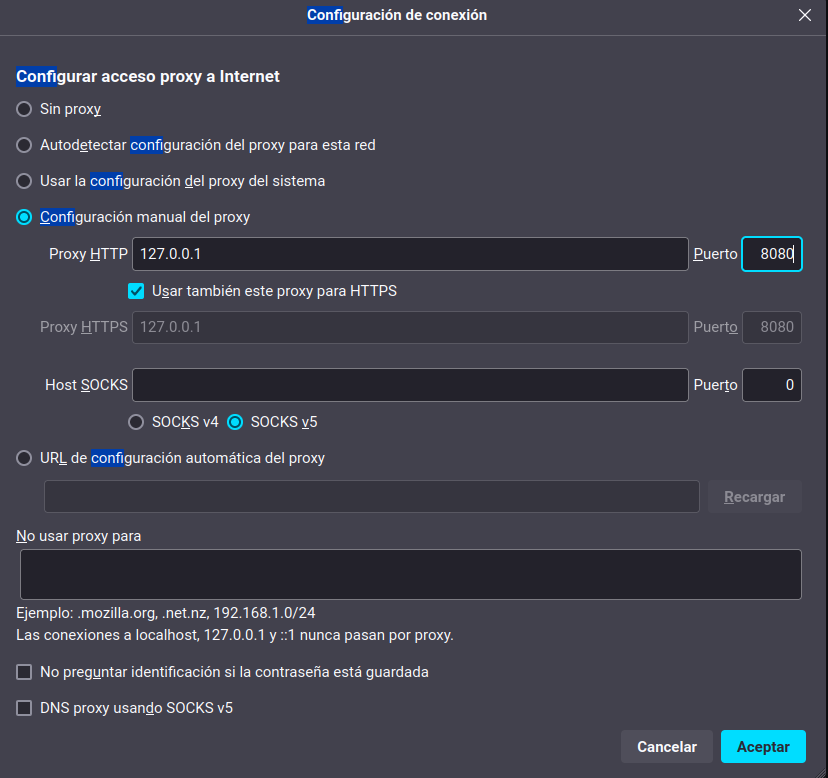
\includegraphics[scale=0.28]{imagenes/Captura desde 2024-05-26 22-28-28.png}
    \end{center}

    Acepta la configuración. Si intentas acceder a alguna web, como por ejemplo \texttt{google.com}, seguramente obtengas el siguiente error:

    \begin{center}
        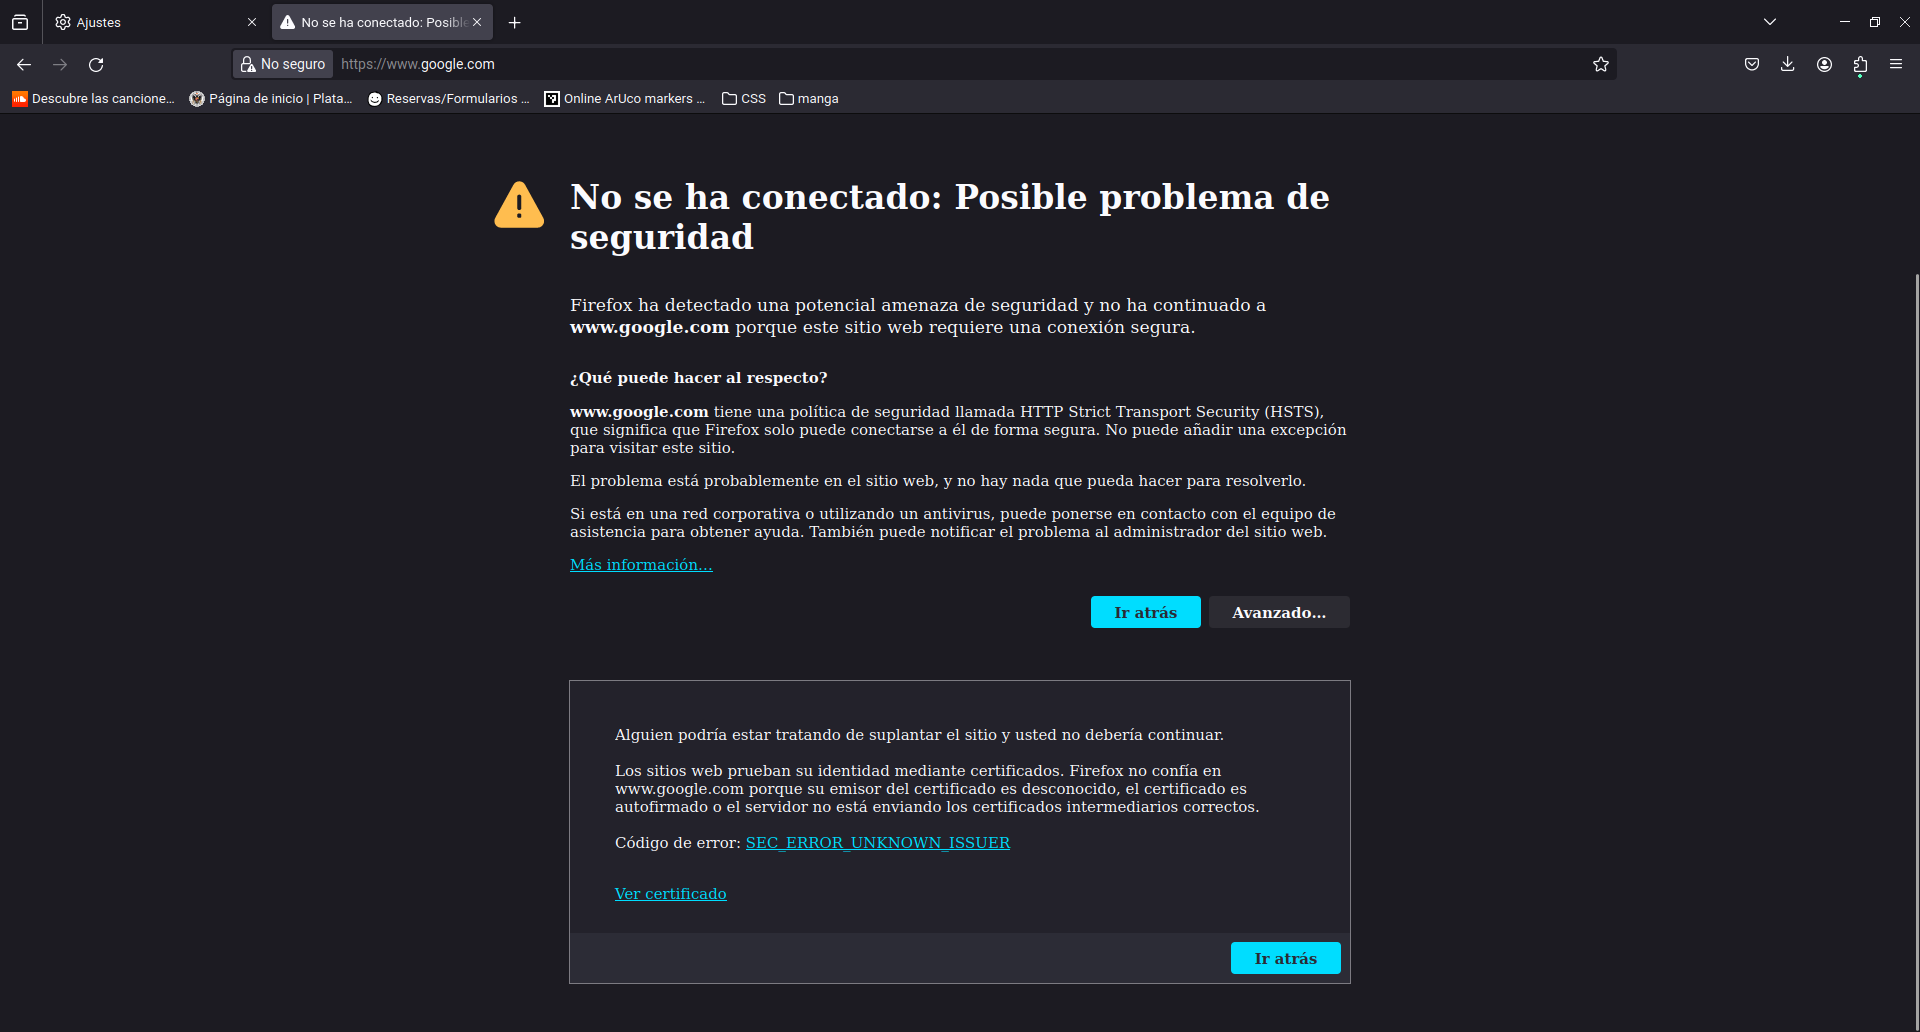
\includegraphics[scale=0.17]{imagenes/Captura desde 2024-05-26 22-22-15.png}
    \end{center}

    \item \textbf{Instalar certificado de \texttt{Burp Suite} en el navegador}: Para arreglar el error anterior, accede a \texttt{http://burp}. Deberías observar una web como la siguiente:

    \begin{center}
        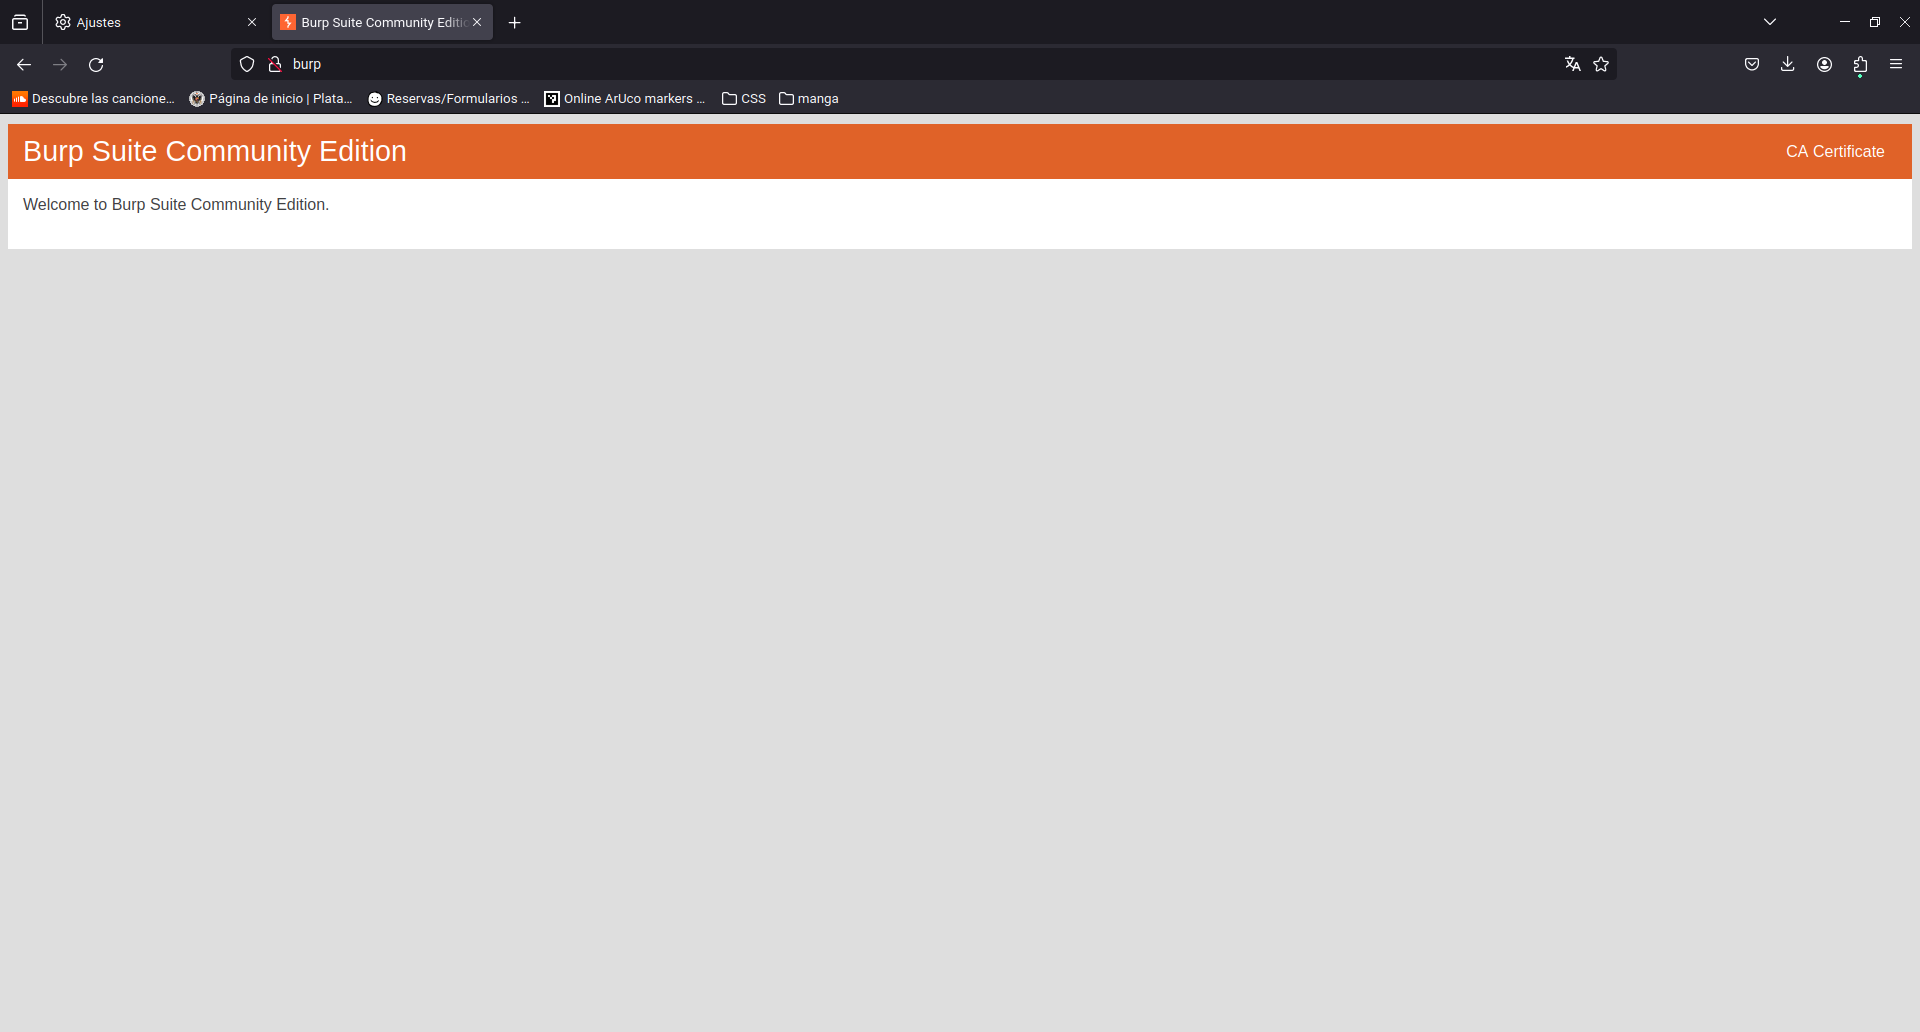
\includegraphics[scale=0.17]{imagenes/Captura desde 2024-05-26 22-22-30.png}
    \end{center}

    Una vez dentro, haz click en el botón para descargar el certificado y, a continuación, ve a \texttt{Ajustes > Certificados} para añadir el certificado al navegador:

    \begin{center}
        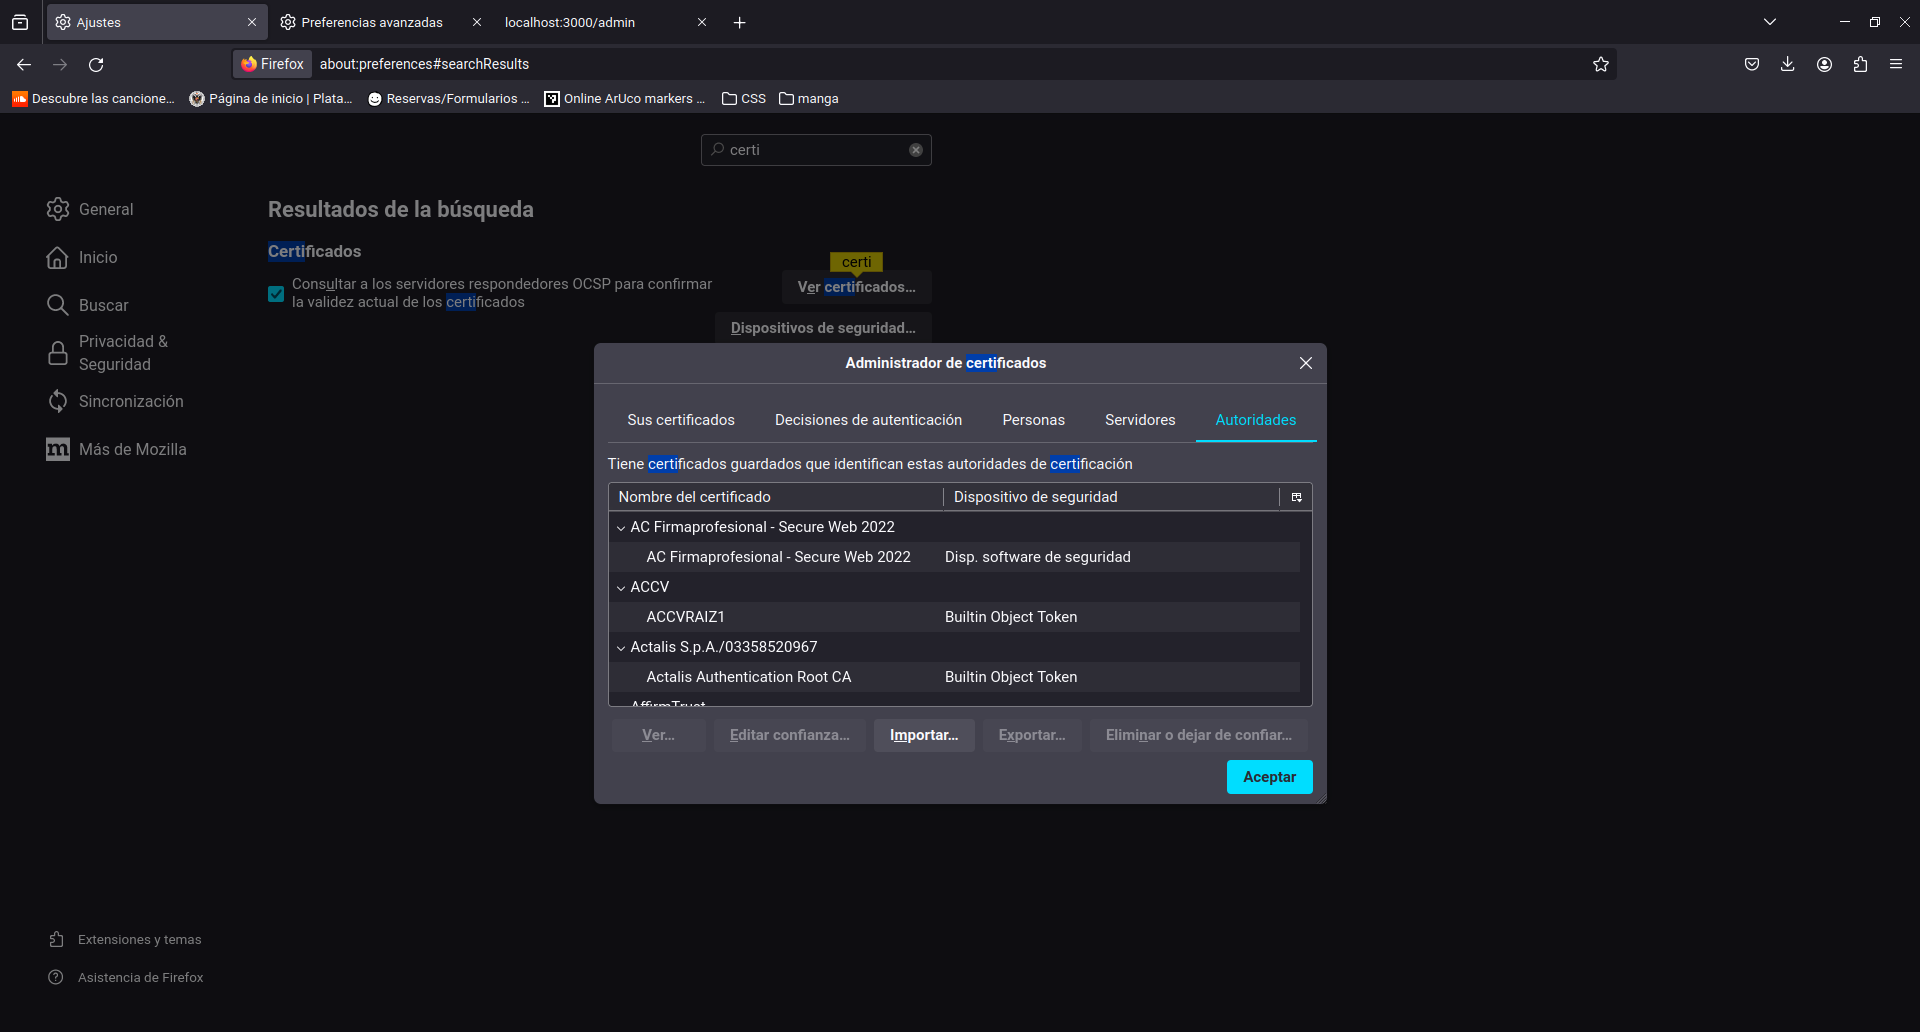
\includegraphics[scale=0.17]{imagenes/Captura desde 2024-05-26 23-44-39.png}
    \end{center}

    Dale a importar, marca todas las casillas y añade el certificado al navegador. Después de esto, podrás navegar de forma normal. Para interceptar las peticiones en \texttt{Burp Suite}, asegurate de que aparezca \texttt{Intercept is on} (\textit{Si no aparece basta con hacer click en \texttt{Intercept is off}}).

    Comprueba que puedes usar el navegador correctamente y que llegan las peticiones a \texttt{Burp Suite}:

    \begin{center}
        \begin{tabular}{l|r}
           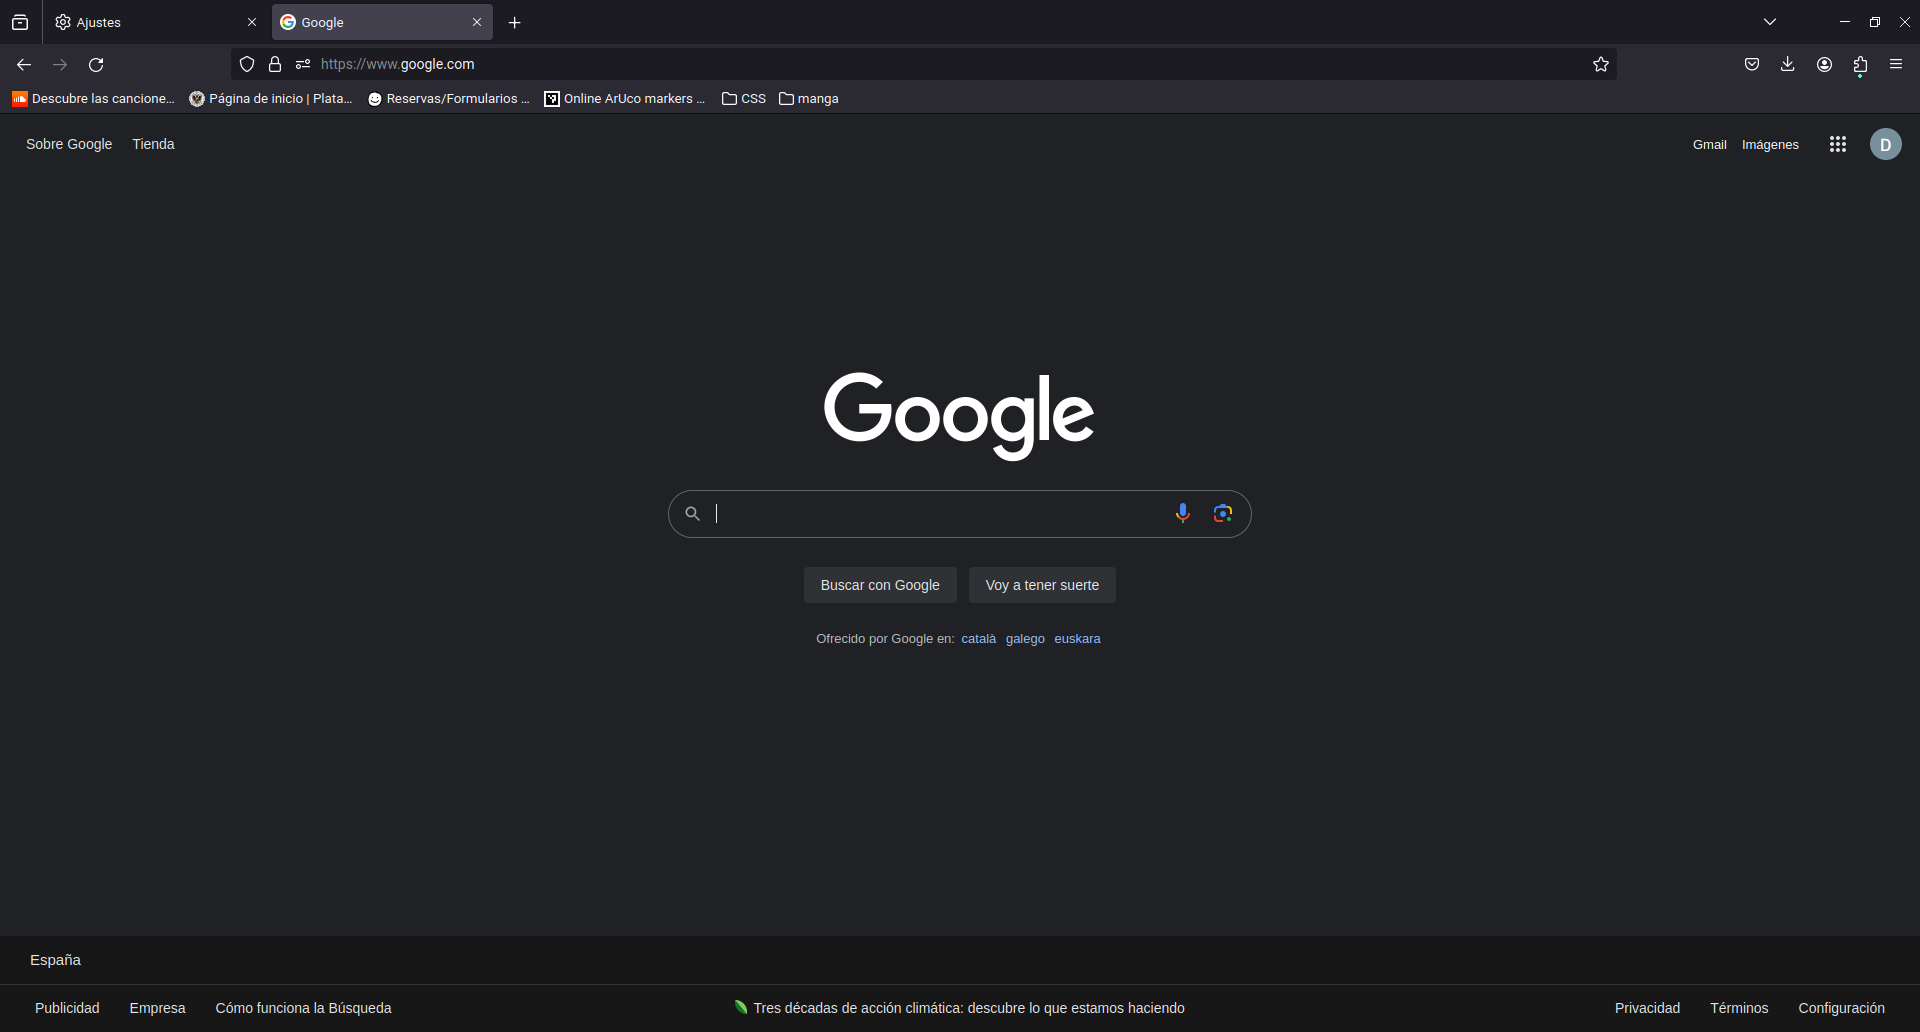
\includegraphics[scale=0.08]{imagenes/Captura desde 2024-05-26 22-23-28.png}  &  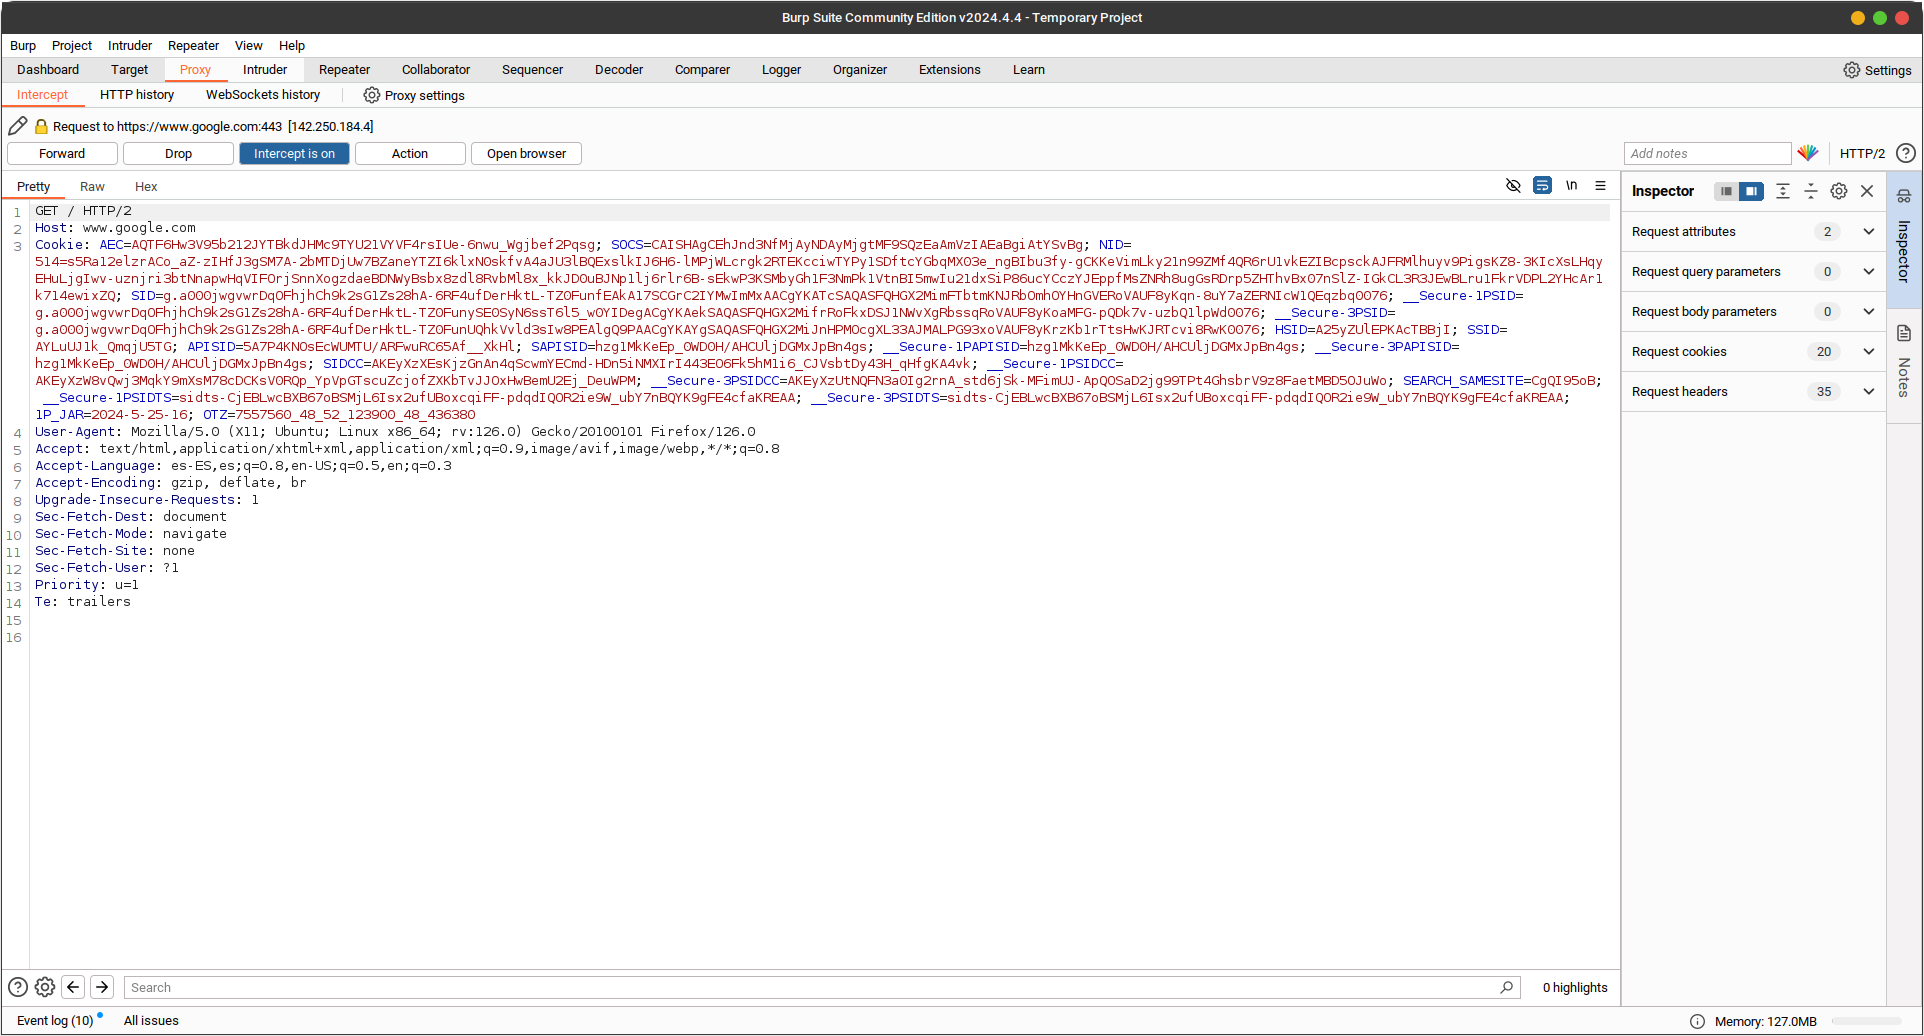
\includegraphics[scale=0.08]{imagenes/Captura desde 2024-05-26 22-23-58.png}
        \end{tabular}
    \end{center}
\end{enumerate}

\textbf{\textit{Es importante que recuerdes deshabilitar estas configuraciones cuando acabes el experimento}}.

Ahora vamos a volver a enviar la solicitud post ~\ref{lst:fetch-post}. Esta vez al ejecutar el código, veremos la siguiente petición \texttt{HTTP} en \texttt{Burp Suite}:

\begin{center}
    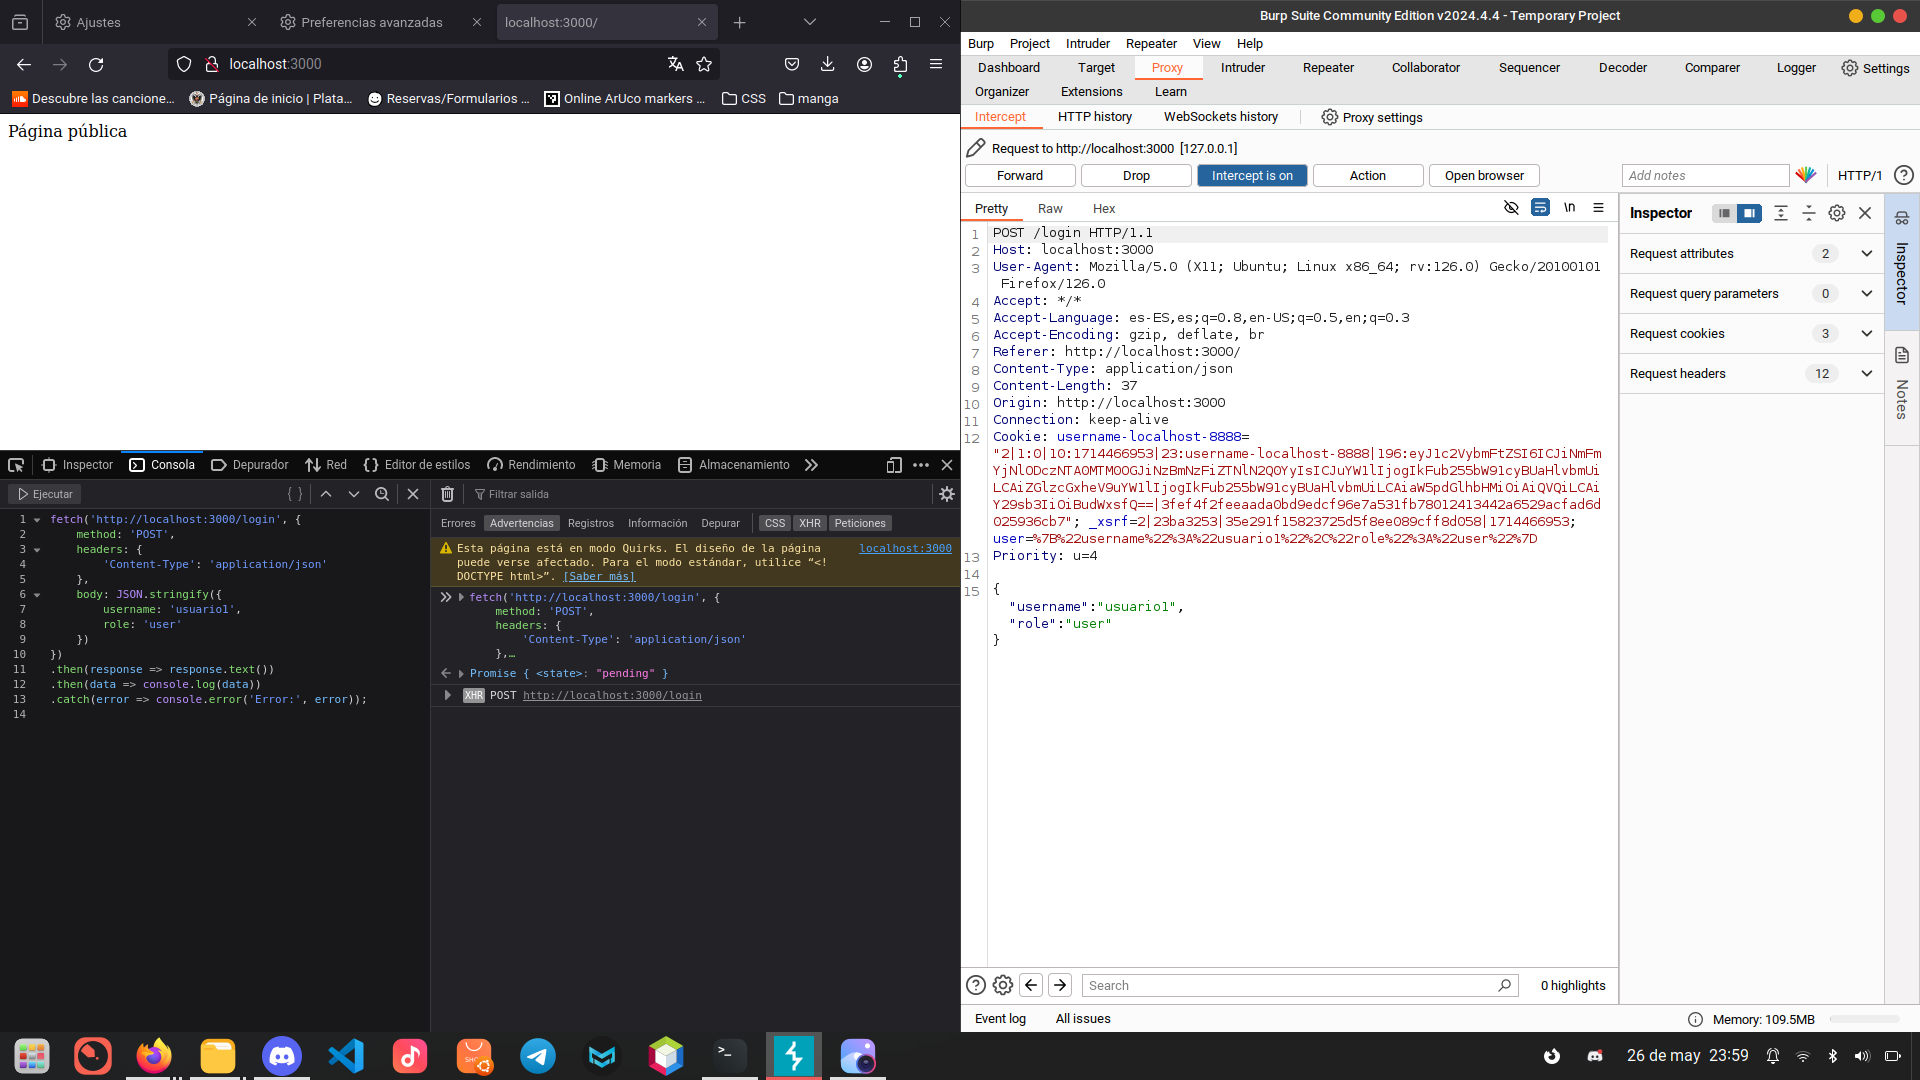
\includegraphics[scale=0.15]{imagenes/Captura desde 2024-05-26 23-59-16.png}
\end{center}

Cambia el valor de ''role'' y establécelo a ''admin''. A continuación, haz click en \texttt{Forward}, lo cuál provocará que la petición se mande con la cookie modificada. Podemos acceder nuevamente a \texttt{http://localhost:3000/admin} para comprobar el resultado:

\begin{center}
    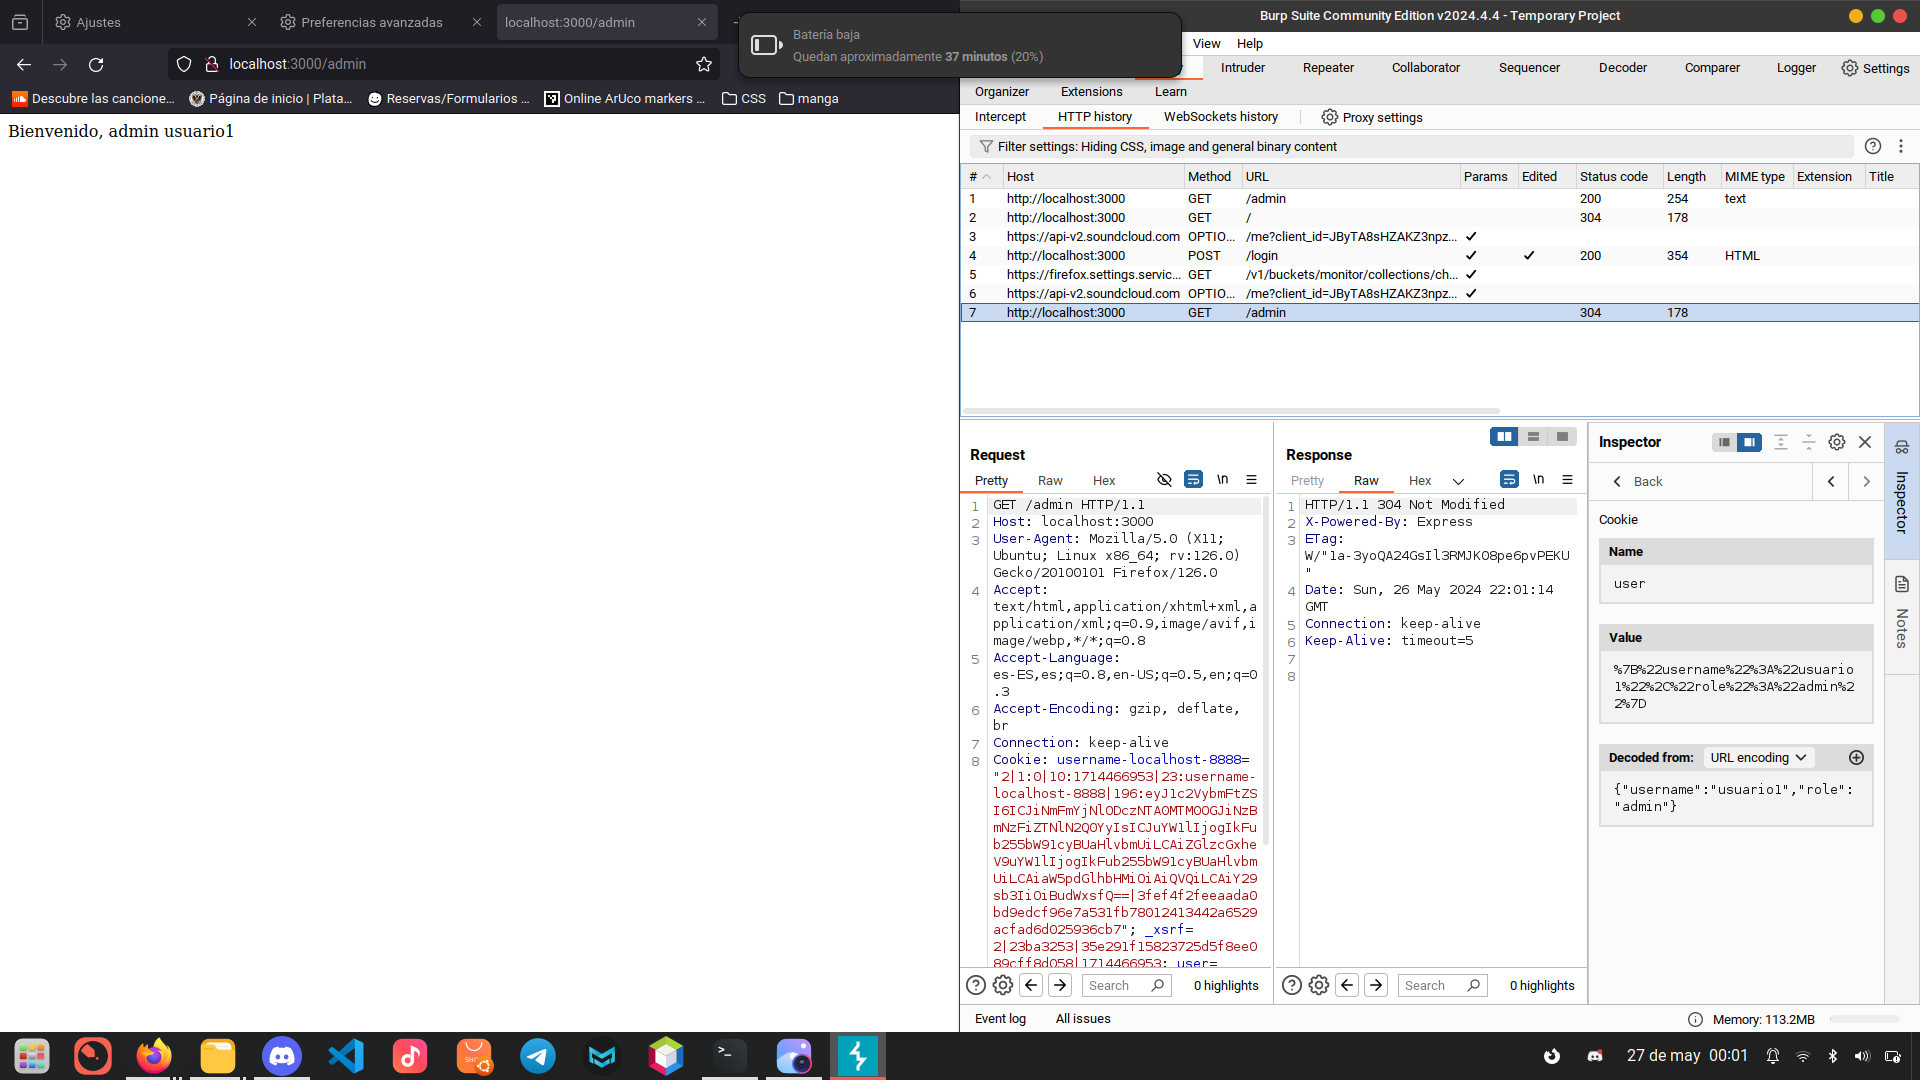
\includegraphics[scale=0.15]{imagenes/Captura desde 2024-05-27 00-01-34.png}
\end{center}
\clearpage
\section{Conclusiones}


En este trabajo, hemos investigado diversas formas de realizar ataques de \textbf{cookie poisoning}, una amenaza que puede parecer poco conocida a priori. Hemos identificado las vulnerabilidades más comunes y las técnicas más efectivas para prevenirlos y detectarlos. A continuación, vamos a presentar las conclusiones más claras que encontramos sobre este y algunas posibles mejoras en la protección frente a estos ataques.


\subsection*{Vulnerabilidades más comunes y prueba práctica expuesta}

Como hemos visto anteriormente, las vulnerabilidades más comunes que permiten el \textit{cookie poisoning} incluyen la falta de validación adecuada de las cookies y la insuficiente implementación de medidas de seguridad, como el uso de cookies HttpOnly y Secure o la falta de cifrado de estas. 

La prueba práctica realizada con \textit{Burp Suite} demuestra claramente cómo es posible modificar el valor de una cookie para obtener acceso a áreas restringidas de una aplicación web. Este pequeño experimento destaca la necesidad de una validación robusta y continua de la integridad de las cookies.

\subsection*{Impacto de estos ataques y recomendaciones finales}

Los ataques expuestos a grandes empresas, como a Yahoo y LastPass, muestran la gravedad y el impacto de estos ataques y resaltan la necesidad de implementar medidas de seguridad para proteger la privacidad y la integridad de los datos de las aplicaciones.

Como recomendación para evitar ataques de \textbf{cookie poisoning}, toda aplicación debería implementar varias medidas de seguridad esenciales. Entre ellas, el cifrado adecuado de las cookies, el uso de la bandera \textit{HttpOnly} y \textit{Secure}, y la validación obligatoria de las cookies en el servidor.

Además, estar al tanto de los últimos desarrollos, como las \textbf{Device Bound Session Credentials (DBSC)} de \textit{Google}, puede otorgar una capa adicional de protección contra el robo de cookies de sesión y el acceso no autorizado a cuentas de usuario.


En conclusión, este tipo de ataques es una amenaza importante para la seguridad de las aplicaciones web, pero con la implementación de las medidas adecuadas y la realización de investigaciones continuas, es posible mitigar estos riesgos y proteger de manera más segura la información de los usuarios.


\clearpage
%
%
% \nocite{*}
\bibliography{bibliografia/bibliografia}\addcontentsline{toc}{section}{Bibliografía}
\bibliographystyle{plainurl}
%
%\appendix
%\input{apendices/manual_usuario/manual_usuario}
%%\input{apendices/paper/paper}
%\input{glosario/entradas_glosario}
% \addcontentsline{toc}{chapter}{Glosario}
% \printglossary
\thispagestyle{empty}

\end{document}
